\documentclass[exercice]{thedocument}%
\startdatakeys
\source{}
\cycle{}
\competencesDuSocle{}
\connaissancesRequises{}
\competencesTravaillees{}
\enddatakeys
\begin{document}%
Calculer l'aire des disques suivants :\par\noindent\vskip10pt
{\bfseries 1)}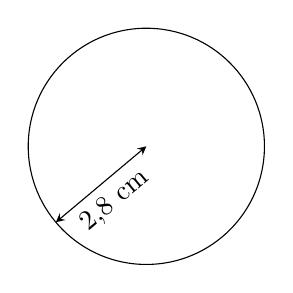
\begin{tikzpicture}[scale=0.5]
    \coordinate(O)at(0,0);
    \draw(O)circle(3);
    \draw[stealth-stealth](O)--(220:3)node
        [pos=0.5,below,sloped]{2,8 cm};
\end{tikzpicture}\hfill
{\bfseries 2)}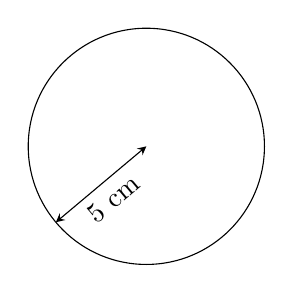
\begin{tikzpicture}[scale=0.5]
    \coordinate(O)at(0,0);
    \draw(O)circle(3);
    \draw[stealth-stealth](O)--(220:3)node
        [pos=0.5,below,sloped]{5 cm};
\end{tikzpicture}\par\noindent\vskip10pt
{\bfseries 3)}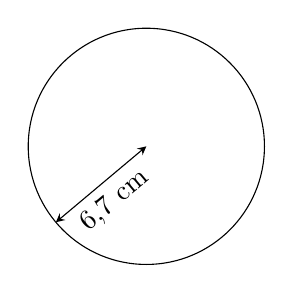
\begin{tikzpicture}[scale=0.5]
    \coordinate(O)at(0,0);
    \draw(O)circle(3);
    \draw[stealth-stealth](O)--(220:3)node
        [pos=0.5,below,sloped]{6,7 cm};
\end{tikzpicture}\hfill
{\bfseries 4)}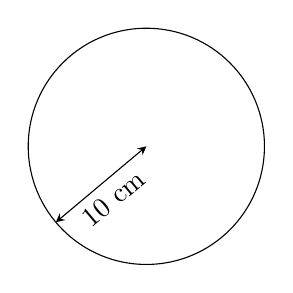
\begin{tikzpicture}[scale=0.5]
    \coordinate(O)at(0,0);
    \draw(O)circle(3);
    \draw[stealth-stealth](O)--(220:3)node
        [pos=0.5,below,sloped]{10 cm};
\end{tikzpicture}
\end{document}
